\chapter{Locally-linear pictorial structures}\label{sec:llps}
\section{Introduction}
\out{
Human pose estimation from single, 2D images holds great potential to assist in 
a wide range of applications---semantic indexing of images and videos, action 
recognition, activity analysis, and human computer interaction, to name a few.
However, human pose estimation ``in the wild'' is an extremely challenging 
problem.  It shares all of the difficulties of object detection, such as 
confounding background clutter, lighting, viewpoint, and scale, in addition to
significant difficulties unique to human poses. 
}

In this chapter, we focus explicitly on the multimodal nature of the 2D pose 
estimation problem.  As discussed in~\secref{perceptual}, there are enormous 
appearance variations in images of humans.  This is due to foreground and 
background color, texture, viewpoint, and body pose.  The shape of body parts 
is further varied by clothing, relative scale variations, and articulation 
(causing foreshortening, self-occlusion and physically different body 
contours).

\begin{figure}[t!]
\centering
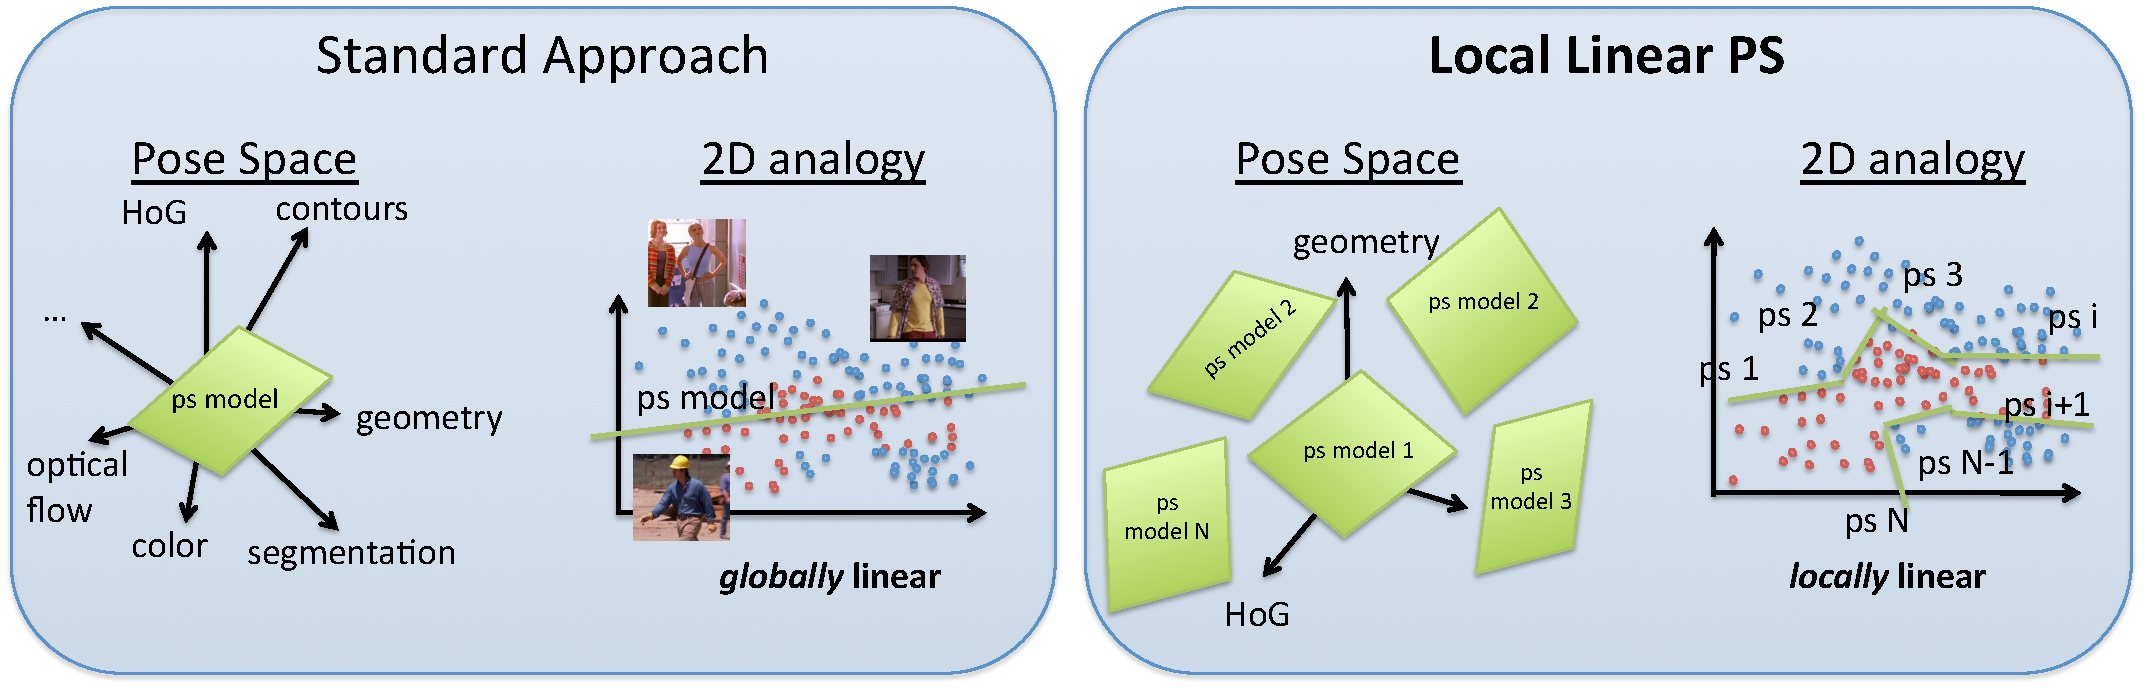
\includegraphics[width=0.99\linewidth]{figs/llps-overview.pdf}
\caption[LLPS overview.]{\label{fig:overview} \textbf{Left:} Most pictorial 
structures researchers have put effort into better and larger feature spaces, 
in which they fit one linear model.  The feature computation is expensive, and
still fails at capturing the many appearance modes in real data.  
\textbf{Right:} We take a different approach.  Rather than introduce an 
increasing number of features in hopes of high-dimensional linear separability, 
we model the non-linearities in simpler, lower dimensional feature spaces, 
using a collection of {\em locally} linear models.}
\end{figure}


Most models developed to estimate human pose in these varied settings use {\em 
only a single, linear model}---\eg, 
\citet{devacrf,eichner09,andriluka09,ddtran} and the models described
in~\secref{CPS} and~\secref{stretchable}.
Such models make it very difficult to capture the part variations discussed.  
Instead, many researchers have focused attention on improving features in hopes 
that a better feature space will make a linear model discriminate correct poses 
from incorrect ones well.  However, this comes at a price of considerable 
feature computation cost---\CPS, for example, requires computation of Pb 
contour detection and Normalized Cuts (see~\secref{features} for details), each 
of which takes minutes.

Recently, especially the past two years, there has been an explosion of  
successful work focused on increasing the number of modes in pose models. This 
line of work in general can be described as instantiations of a {\em family of 
compositional, hierarchical pose models}.  The family of models can be 
parametrized by the number of {\em part levels } and the number of {\em part 
modes} captured per part.  The part levels can encode different granularities 
and scope of pose---\eg, {\em \{ wrist, lower arm, full arm, half-body, full 
body \}} are example parts in a 5-level hierarchy.  The higher-level parts can 
leverage more image context but must generalize larger within-mode variations 
in pose.  They serve to inform lower-level parts of likely locations.  Part 
modes at any level can capture different poses (\eg, elbow crooked, lower arm 
sideways) and appearance (\eg, thin arm, baggy pants).  Also of crucial 
importance are details such as how models are trained, the computational 
demands of inference, and how modes are defined or discovered.  Details for all 
recent work is in \tabref{rel-work-ps}, which we discuss at length in 
\secref{llps-rel}.


\mypar{Our approach:} In this chapter, we propose a particular instantiation of 
a multimodal model with a focus on simplicity, speed and accuracy.  We capture 
multimodality at the global level, which gives us the ability to capture a 
variety of pose modes, each modeled as a discriminative linear classifier.  
Thanks to the rich, multimodal nature of the model, we see performance 
improvements even with only computationally-cheap image gradient features.  

The model features an explicit mode selection variable, the value of which is 
jointly inferred along with the best layout of body parts in the image at test 
time.  Unlike some previous work, our method is trained jointly (thus avoiding 
difficulties calibrating different submodel confidences) and includes both 
holistic and local part-level cues (thus allowing it to effectively predict 
which mode to use).  Finally, we employ an initial structured cascade mode 
selection step which cheaply discards unlikely modes up front, yielding a 
$5\times$ speedup in inference and learning over considering all modes for 
every example.  This makes our model faster than state-of-the-art approaches 
(on average, 1.31 seconds vs. 1.76 seconds for \citet{deva2011}), while being 
significantly more accurate.  It also suggests a way to scale up to even more 
modes as larger datasets become available.
 

\section{Related work}\label{sec:llps-rel}
 \begin{table}[bt!]
\begin{center}
{\small
\begin{tabular}{| r | c | c |c | c | c | c | c |}
\hline
model &	atomic unit & part levels & training obj. & \# global modes	& \# part modes	& graph type & latent modes?	\\
\hline
basic ps	& limbs	& 1 &	parsing	& 1	& 1	& tree & no \\
\cite{wang2008multiple} & limbs & 1 &	parsing &	3	& 1	& tree &	no \\
\cite{everingham2011} &	limbs &	1 &	parsing &	16 & 4* &	tree &	yes \\
\cite{deva2011} &	joints & 1	& detection &	1 &	4 to 6 & tree	& yes \\
\cite{wang2011} & limbs & 4	& parsing	& 1 &	5 to 20 & cyclic & no \\
\cite{sun2011} & limbs	& 4	&	parsing	& 1	& 4	& tree & yes \\
\cite{ramanan-faces} &	joints &	1	& detection &	18	& 1** &	tree	& yes \\
\cite{batra2012} & joints	& 4	&	detection &	9 &	4 to 6 & cyclic &	no \\
\cite{tianexploring} & limbs & 3 & detection	& 5 &	5 to 15 &	tree & yes \\
\hline
OURS & joints & 2 & both & 32 & 1 & tree & no \\
\hline
\end{tabular}



}
\end{center}
\footnotesize{ * Part modes are not explicitly part of the state, but instead 
are maxed over to form a single detection.\\  ** A variety of parameter sharing 
across global models is explored, thus there is some multimodal information 
used during training. }
\caption[Family of multimodal pose models.]{In the past few years, there have 
been many instantiations of the family of multimodal models. The recent models 
listed here and their attributes are described in the text. \\
}
\label{tab:rel-work-ps} \end{table}

We discuss here in depth the differences in recent works concerning multimodal 
models of pose.  We then briefly go into other related models in the computer 
vision and machine learning communities.

\subsection{Multimodal modeling}
As can be seen in \tabref{rel-work-ps}, compositional, hierarchical modeling of 
pose has enjoyed a lot of attention recently.  In general, works either 
consider only global modes, local modes, or several multimodal levels of parts.

\mypar{Global modes but local cues.} Some works consider models with a number 
of distinct global modes \citep{everingham2011,ramanan-faces,wang2008multiple}, 
enumerating over tens of disjoint models and taking the highest scoring.  One 
characteristic of all previous models in this category is that they only employ 
local part cues (\eg wrist patch or lower arm patch), making it difficult to 
adequately represent and predict the best global mode.  A second issue is that 
some sort of model calibration is required, so that scores of the different 
models are comparable.  One way to do this is to train the models jointly by 
explicitly reasoning over a mode variable, as we do in our model.  
\citet{everingham2011} instead calibrate the models post-hoc using 
cross-validation data, similar to \citet{esvm}.

\mypar{Local modes.} A second approach is to focus on modeling modes only at 
the part level, \eg \citet{deva2011}.  If $n$ parts each use $k$ modes, this 
effectively gives up to $k^n$ different instantiations of modes for the 
complete model through mixing-and-matching part modes.  Although 
combinatorially rich, this approach also lacks the ability to reason about 
larger structure, not just from lack of global cues, but the inability of the 
representation to reason about larger structures such as global modes.  A 
second issue is that to reason about a pair of neighboring nodes, one must 
consider a quadratic number of local mode combinations---\eg for each of $k$ 
wrist types, $k$ elbow types must be considered, resulting in inference message 
passing that is $k^2$ larger than unimodal inference.

\mypar{Additional part levels.}
A third category of models consider both global, local and intermediate level 
modes \citep{wang2011,sun2011,batra2012,tianexploring}.  At all levels, cues 
for the level are used, allowing the model to effectively capture mode 
information at different levels of part granularity.  The biggest downside to 
this approach is that it is slow:  First, quadratic mode inference is 
necessary, as with any local mode modeling.  Second, inference grows linearly 
with the number of additional parts, and becomes intractable when part 
relations are cyclic, as in \citet{wang2011, batra2012}.

\mypar{Defining modes.}
The mode definitions are typically obtained by clustering in the space of part 
configurations.  \citet{everingham2011} include appearance in the definition of 
a mode.  In roughly half of the previous literature, local modes are considered 
latent variables to be re-estimated during training.  This renders otherwise 
convex learning formulations non-convex, iterative learning procedures, where 
good mode initialization is crucial to converge to a good local minima.


\mypar{Contrast with our model.}
In contrast to the above, our model supports multimodal reasoning at the global 
level, as in \citep{everingham2011,ramanan-faces,wang2008multiple}.  Unlike 
those, we explictly reason about, represent cues for, and jointly learn to 
predict the correct global mode as well as location of parts.  Unlike local mode models such as 
\citet{deva2011}, we do not require quadratic part-mode inference and can 
reason about larger structures.  Finally, unlike models with additional part 
levels, ours is fast: a simple two-level model with no local modes and 
tractable inference.  This also relieves us of the guesswork inherent in 
learning latent modes. We also apply a structured prediction mode filtering 
step to reduce the number of modes considered for each test image. 

\subsection{Other models}
\mypar{Throwing features at the problem:} Equipped with a linear model of human 
pose, most researchers focus attention instead on increasing the quality of 
features, to be robust to the variety of modes discussed 
above---lighting-invariant texture modeling~\citep{andriluka09}, foreground and 
skin color~\citep{devacrf,eichner09}, left-right appearance 
similarity~\citep{ddtran,sapp2011}, contour and segmentation 
support~\citep{sapp2010cascades,sapp2011}, and more detailed description of 2D 
geometry~\citep{ddtran,sapp2011}, to name a few.  The hope in all of these 
models is that a linear model in a larger-dimensional feature space will be 
better able to separate the true pose configurations from false alarms, and 
mitigate the issue of non-linearity in lower-dimensional feature spaces, \eg, 
using only edge orientation information.

\mypar{Other local modeling methods:}
In the machine learning literature, there is a vast array of local methods for 
prediction.  Many of these require costly parameter estimation at test time, 
such as locally weighted logistic regression and KNN-SVM~\citep{zhang06}.  
Although we call our method locally linear, it does not estimate parameters at 
test time like these techniques.

Different from those, nearest-neighbor methods are powerful, but live and die 
by the right choice of distance function.  Standard norms fare poorly in 
high-dimensional spaces.  Learning distance functions for nearest neighbors has 
achieved some success, \eg Large-Margin KNN~\citep{lmknn}, which seeks to learn 
a global distance function for the whole sample space.  A refinement of this is 
to learn local distance functions---~\citep{frome07} and the recent 
Exemplar-SVM~\citep{esvm} both learn distance functions per example.  These 
works are quite similar in spirit to ours, but focus on object classification 
and detection, not structured, articulated part localization.


\section{\LLPS}\label{sec:llps-model}

We pose the problem of 2D human pose estimation as a structured prediction 
task.  Let $x$ represent a given input image, and $y$ represent the location of 
$P$ parts in image coordinates.  Each variable $y_i$ denotes the pixel 
coordinates (row, column) of part $i$ in image $x$.  For ``parts'' we choose to 
model joints and their midpoints (\eg, left wrist, left forearm, left elbow) 
which allows us fine-grained encoding of foreshortening and rotation, as is 
done in~\citep{deva2011,sapp2011}.

The standard pictorial structures model described in~\secref{ps} is a linear 
model which decomposes into a sum of unary and pairwise linear terms.  We 
choose a general pairwise MRF form in which the score for a part configuration 
specified by $y$ in image $x$ is:
\begin{align}
 s(x,y) = \sum_{i \in \cV} \w_i \cdot \f_i(x,y_i) + \sum_{(i,j) \in \cE} 
\w_{ij} \cdot \f_{ij}(x,y_i,y_j),
 \label{eq:llps-ps}
\end{align}
When the graph $G = (\cV,\cE)$ describes a tree, we can use efficient dynamic 
programming techniques to infer the best scoring configuration of all parts 
(~\secref{inference}), $y^\star = \argmax_{y \in \mathcal{Y}} s(x,y)$.
The set $\mathcal{Y}$ denotes the entire set of possible poses, which is 
exponential in the number of model parts: $|\mathcal{Y}| = |\mathcal{Y}_i|^P$, 
where $\mathcal{Y}_i$ is the set of possible placements of part $i$ in the 
image (and is the same for all $i$).

% \subsection{\LLPSlong~(\LLPS)}
Instead of a single, linear model as in~\equref{llps-ps}, we model human pose 
with a collection of linear models which describe different local 
neighborhoods.  Let us consider $M$ such models, which we index $z = 1 \ldots 
M$:
\begin{align}
s^z(x,y) = \w^z \cdot \f(x,z) +  \sum_{i \in \cV} \w^z_i \cdot \f_i(x,y_i,z) + 
\sum_{(i,j) \in \mathcal{E}} \w^z_{ij} \cdot \f_{ij}(y_i,y_j,z),
\end{align}
These submodels include the additional, global term $\w^z \cdot \f(x,z)$ which 
help discriminate the submodels from others using global features of the image.  
Each model shares the same tree structure $\mathcal{E}$ for the sake of 
simplicity; it is easy to extend this to a heterogenous collection of tree 
models.  Note the pairwise term we express only as a function of the 
state-space, which allows us to perform inference linear in each part's 
state-space using a distance transform (\secref{dt}).  The $M$ models' 
parameters $\w^z = [\w^z_i;~\w^z_{ij}]$ are learned to fit a local neighborhood 
around each mode center, discussed in~\secref{llps-learning}.

At test time, the full \LLPS models infers both the best local model $z$ to 
use, and the best placement of joints given the corresponding submodel:
\begin{align}
s(x,y,z) &= s^z(x,y) \\
z^\star,y^\star &= \argmax_{z \in [1,M],~y \in \mathcal{Y}} s(x,y,z) 
\end{align}
Thus, given a test example, the test time inference procedure is 
straightforward: evaluate all $M$ local submodels (in practice, we use 32 modes 
for upper body pose estimation), via max-sum inference (\secref{inference}), 
saving the score and highest scoring output sequence of each.  Then, we take 
the highest scoring of the $M$ local models and its output sequence as a 
prediction of the pose.  This procedure is linear in $M$.  In the next section 
we show a superlinear speedup using cascaded prediction.

\subsection{Cascaded mode filtering}

The use of structured prediction cascades has been a successful tool for 
drastically reducing state spaces in structured problems.  In \secref{CPS} and 
\secref{stretchable}, the cascade method was used to reduce
the number of locations to consider for human parsing.  Here we employ a simple 
multiclass cascade step to reduce the number of modes considered in the full 
$\LLPS$ model. We employ a cascade model of the form \begin{align}
c(x,z) = \theta^z \cdot \phi(x,z)
\end{align}
whose purpose is to score the mode $z$ in image $x$, in order to filter 
unlikely mode candidates.  The features of the model are $\phi(x,z)$ which 
capture the pose mode as a whole instead of individual local parts, and the 
parameters of the model are a linear set of weights for each mode, $\theta^z$.  
Following the cascade framework, we retain a set of mode possibilities $\bar{M} 
\subseteq [1,M]$ after applying the cascade model:
\begin{align}
\bar{M} = \{ z \;|\; c(x,z) \geq \alpha \max_{z \in [1,M]} c(x,z) + 
\frac{\alpha-1}{M} \sum_{z \in [1,M]} c(x,z) \}
\end{align}

The metaparameter $\alpha \in [0,1)$ is set via cross-validation and dictates 
how aggressively to prune---between pruning everything but the max scoring mode 
to pruning everything below the mean score.  Applying this cascade before 
running the final level \LLPS model results in the inference task
\begin{align}
z^\star,y^\star &= \argmax_{z \in \bar{M},~y \in \mathcal{Y}} s(x,y,z) 
\end{align}
where $|\bar{M}|$ is considerably smaller than $M$.  In practice it is on 
average $5$ times smaller, giving us a $5\times$ speedup.

\begin{figure}[tb!]
\centering
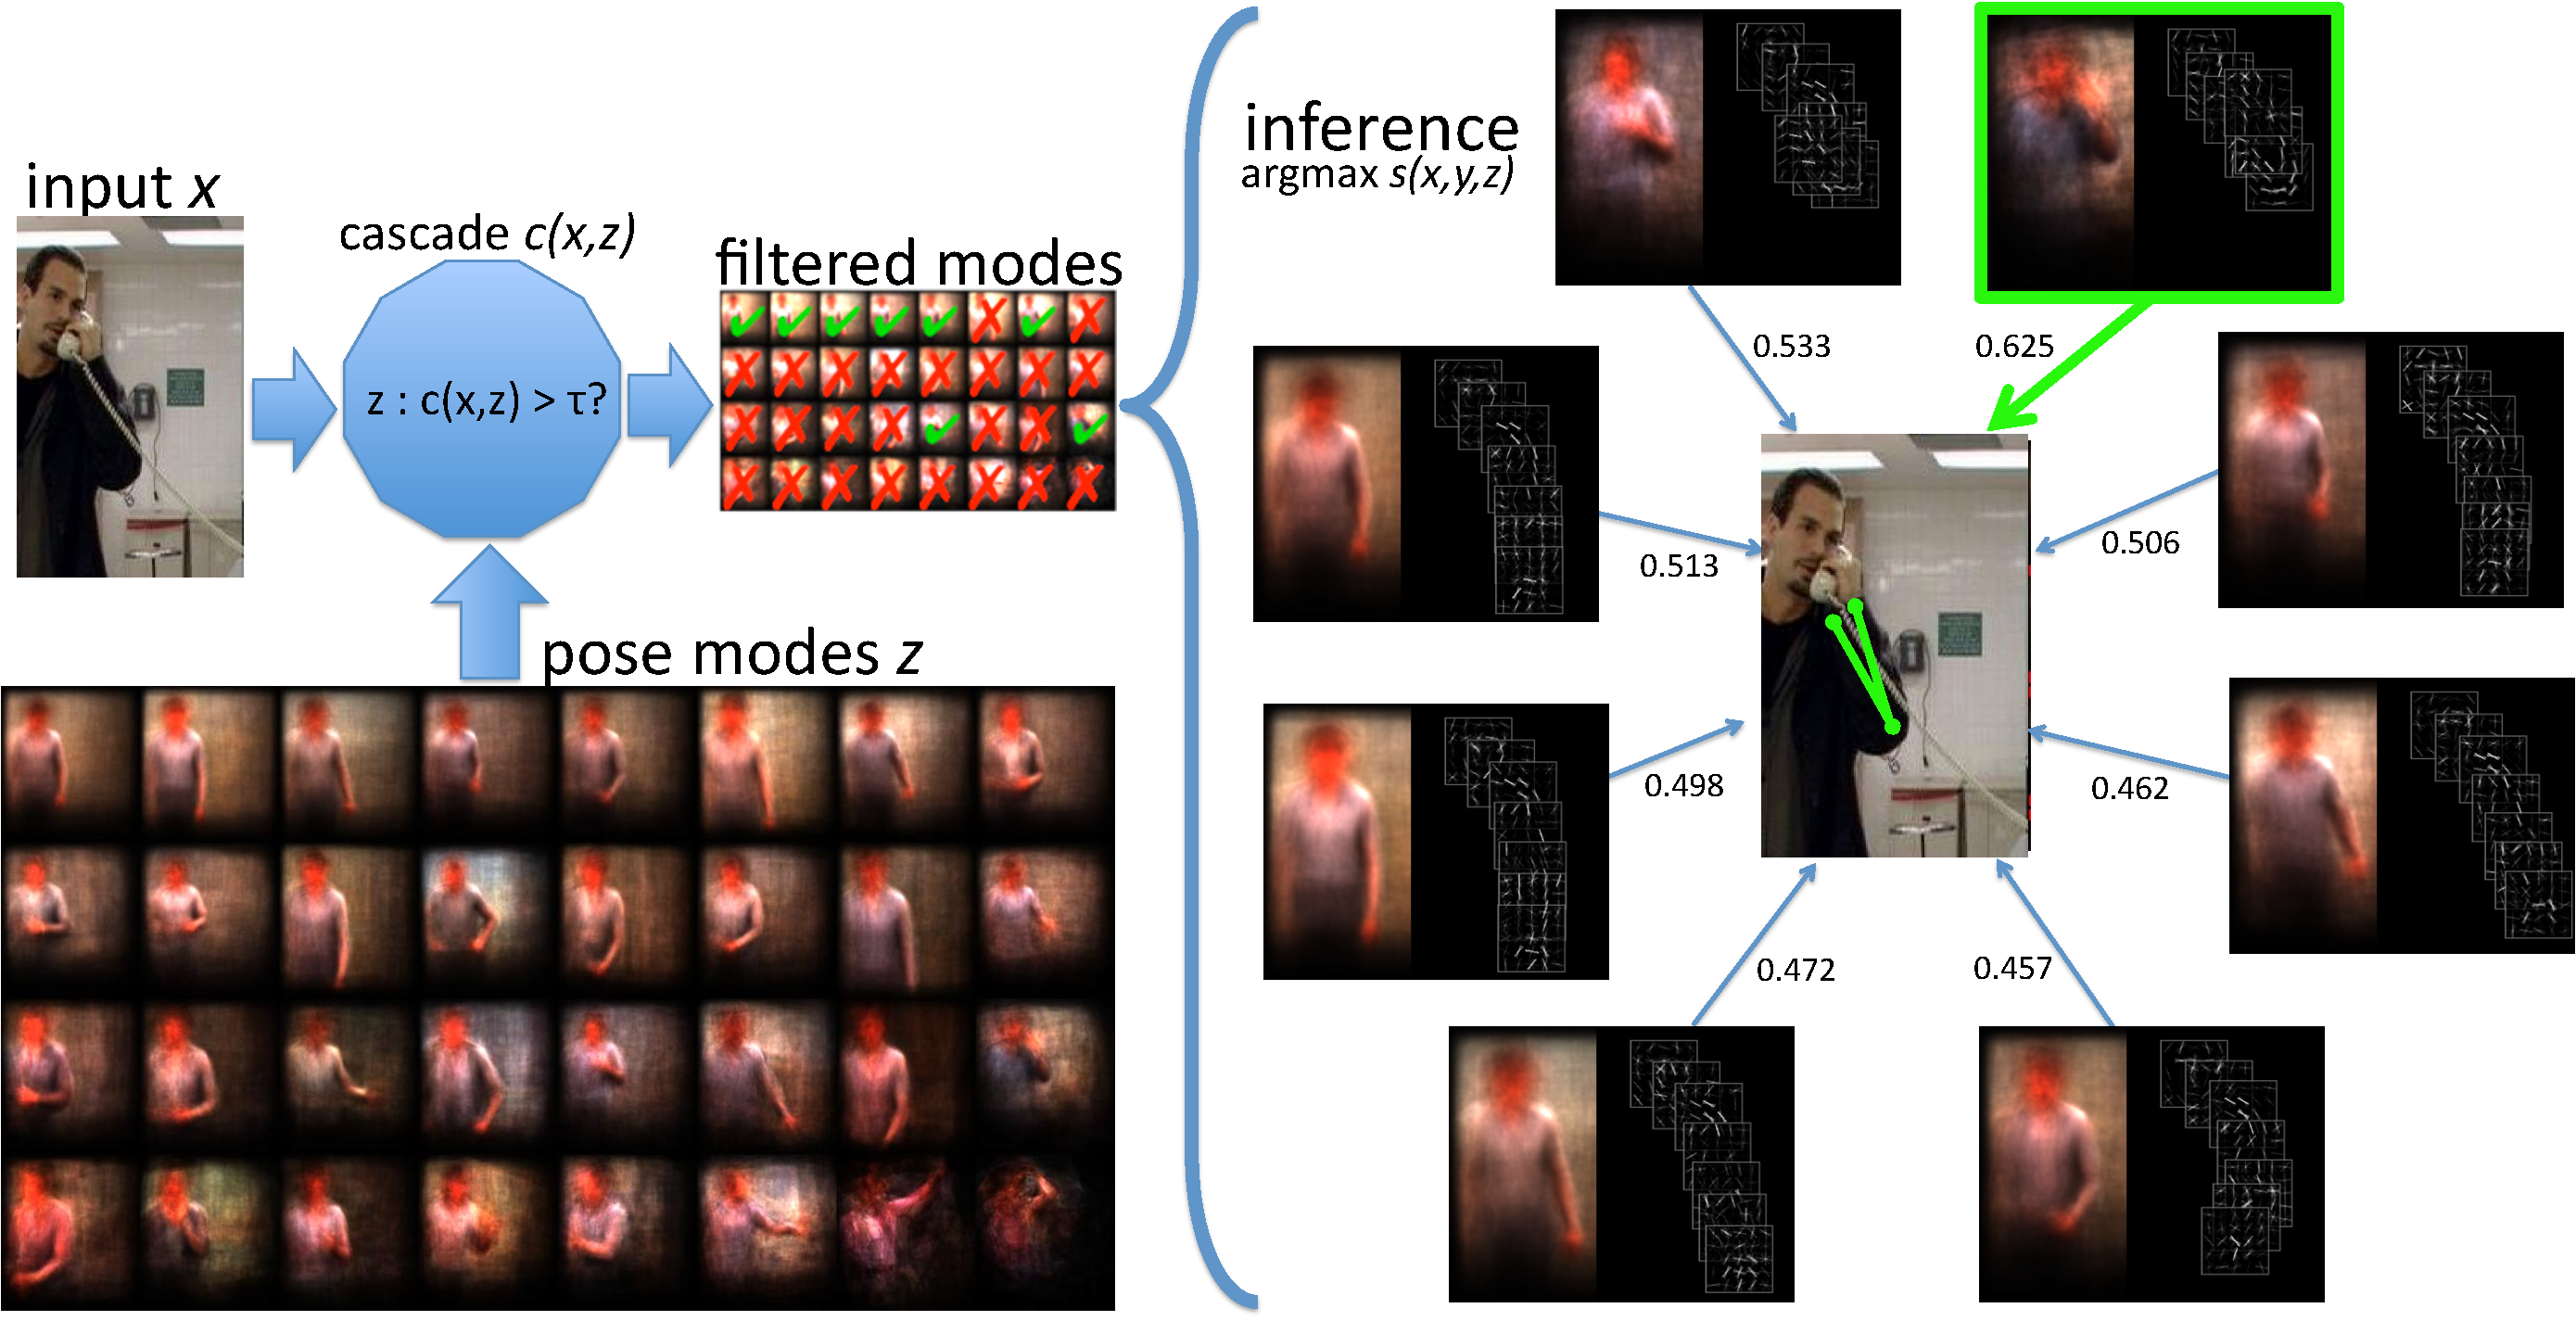
\includegraphics[width=0.99\linewidth]{figs/llps-overview-example.pdf}
\caption[LLPS inference.]{\label{fig:llps-inference} An illustration of the 
inference process. First, modes are cheaply filtered via a cascaded prediction 
step.  Then each remaining local submodel can be run in parallel on a test 
image, and the argmax prediction is taken as a guess. }
\end{figure}
The full system pipeline is laid out in \figref{llps-inference}.  Given an 
input image, we first quickly discard most of the possible modes via the 
cascade model.  The remaining  modes are then each applied independently on the 
test image.  The models are trained jointly and thus their inference scores are 
well-calibrated.  We take the highest scoring position of part layout $y$ from 
submodel/mode $z$ as the final prediction.

\subsection{Image-adaptive pose priors and a non-parametric perspective}
One important perspective of the above is as a mode {\em switching model}, 
popular in speech synthesis \citep{rosti2003switching}.  In this setting, $z$ 
can be thought of as a switch which chooses between different appearance and 
pose priors.  The particular instantiation of $z$ depends on the image content.  
This is related to another, locally-linear method called Adaptive Pictorial 
Structures (APS) \citep{sapp2010}.  In this work, the pose prior terms 
$\f_{ij}$ were adjusted based on a kernel-weighted sum of exemplar similarities 
to the image.  \LLPS, on the other hand, forces a discrete choice from a 
dictionary of pose priors, and this procedure is learned discriminatively.  
From a more practical standpoint, APS relied on very costly and heuristic 
nearest-neighbor computation.  It searched densely through a large number of 
deformations to handle articulation, rather than making use of a structured 
decomposable similarity (\ie, the \LLPS submodel scores).  Each submodel of 
\LLPS can be thought of as a decomposable similarity function, learned 
discriminatively to separate true poses from wrong ones locally, as we will see 
next.

\section{Learning}\label{sec:llps-learning}

During training, we have access to a training set of images with labeled poses 
$\cD = \{(x^{t},y^{t})\}_{t=1}^T$.  As described, we choose to model a local 
neighborhood in pose and appearance centered around predefined modes in pose 
space.  This allows us to capture fine variations of appearance and part layout
due to pose.

\mypar{Mode definitions.}
Modes are obtained from the data by finding centers $\{\mu_i \}_{i=1}^M$ and 
example-mode membership sets $S = \{S_i\}_{i=1}^M$ in pose space that minimize 
reconstruction error under squared Euclidean distance:
\begin{align}
S^\star = \argmin_{S} \sum_{i=1}^M \sum_{t \in S_i} ||y^{t} - \mu_i||^2
\end{align}
where $\mu_i$ is the Euclidean mean of the examples in mode cluster $S_i$.  We 
approximately minimize this objective with the $k$-means algorithm with 100 
random restarts.  We take the cluster membership as our supervised definition 
of mode membership in each training example, so that we augment the training 
set to be $\cD = \{(x^t,y^t,z^t)\}$. 

 \mypar{Parsing constraints.} We seek to learn to correctly identify the 
correct mode {\em and } location of parts in each example.  Intuitively, for 
each example this gives us hard constraints of the form \begin{align}
s^{z^t}(x^t,y^t) - s^{z^t}(x^t,y') &\geq 1,\; &\forall y' \neq y^t 
\label{eq:c1} \\
s^{z^t}(x^t,y^t) - s^{z'}(x^t,y) &\geq 1 ,\; &\forall z' \neq z, \forall y 
\label{eq:c2}
\end{align}
In words,~\equref{c1} states that the score of the true configuration for local 
model $z$ must be higher than $z$'s score for any other (wrong) configuration 
in example $t$---the standard max-margin parsing constraint for a single model.  
\equref{c2} states that the score of the true configuration for $z$ must also 
be higher than any score a ``stranger'' model $z'$ has for any pose 
configuration in example $t$.  We refer to these constraints as {\em parsing
constraints} as they deal with scoring the correct parse $y^t$ above others in 
a single example $t$.

\mypar{Detection constraints.} A popular variant recently in the pose 
estimation literature is to use detection-style constraints instead of parsing 
constraints; enforcing the notion that the model score should be low when no 
valid parse exists in images without people 
\citep{deva2011,batra2012,tianexploring}.  These are typically encoded as
\begin{align}
s^{z^t}(x^t, y^t) &\geq +1 &\forall t \\
s^{z}(x^{neg}, y) &\leq -1 &\forall x^{neg} \in \cD^{neg}, \forall y,z
\end{align}
where now $\cD = \cD^{pos} \cup \cD^{neg}$, with $\cD^{neg}$ a database of unannotated images with no people in them.  
Simply put, these constraints enforce that groundtruth parses should have a 
score at least 1, and parses on negative images from any model should score at 
most $-1$.  Notably absent from these constraints is an explicit way to calibrate 
different submodels $z$ with each other as in \equref{c2}.  This type of 
calibration is typically done in a post-hoc heuristic manner, \eg 
\citep{everingham2011,esvm}.  

Detection-style constraints are easily put into our framework by adding a 
negative class mode $z^{neg}$ modeled with a single constant feature.  Then 
$s^{z^{neg}}(x,y) = \tau^{neg}$ is a learned scalar threshold for the negative 
class, and for cases when $z^t$ or $z^{t'} = z^{neg}$, \equref{c2} can be interpreted as
detection constraints
\begin{align}
s^{z^t}(x^t,y^t) &\geq \tau^{neg}+1,\;\; &\forall t \in \cD^{pos}, \label{eq:cneg1} \\
s^{z}(x^{neg},y) &\leq \tau^{neg}-1,\;\; &\forall x^{neg} \in \cD^{neg}, \label{eq:cneg2}
\forall y,z
\end{align}

\mypar{Learning formulation.}
We consider all constraints from \equref{c1} and \equref{c2}, and include a 
negative mode $z^{neg}$ to incorporate detection constraints of the form in 
\equref{cneg1} and \equref{cneg2}.  Adding slack and regularization on the parameters, we get a 
convex, large-margin structured loss jointly over all $M$ local models

\begin{align}\label{eq:full-learn}
&\min_{\{\w^z\}, \{\xi_{t}\}} \;\; \frac{1}{2} \sum_{z=1}^M ||\w^z||_2^2 + 
\frac{C}{T} \sum_{t=1}^T \xi_t \\
&\text{\bf{subject to:} } \\
&s^{z^t}(x^t,y^t) - s^{z^t}(x^t,y') \geq 1 - \xi_t\;\; &\forall y' \neq y^t \\
&s^{z^t}(x^t,y^t) - s^{z'}(x^t,y)  \geq 1 - \xi_t\;\; &\forall z' \neq z \in 
\bar{M}^t, \forall y \end{align}
Note the use of $\bar{M}^t$, the subset of modes unfiltered by our mode 
prediction cascade for each example.  This is considerably faster than 
considering all $M$ modes in each training example. 

The number of constraints listed here is prohibitively large: in even a single 
image, the number of possible outputs $y' \in \cY$ is exponential in the number 
of parts.  Standard techniques to minimize structured SVM objectives like this 
are stochastic gradient descent and cutting plane methods.  We use a cutting 
plane technique where we find the most violated constraint in every training 
example via structured inference.  We then solve \equref{full-learn} under the 
active set of constraints using fast off-the-shelf QP solver 
LIBLINEAR~\citep{liblinear}.  

\section{Modeling human pose with \LLPS}
In~\secref{llps-model} and~\secref{llps-learning}, we detailed a general 
learning and inference framework for local linear structured models.  We now 
fill in necessary details on the graph structure, neighborhood function, and 
features to describe how we apply this model to human pose estimation.
\subsection{Local graph structure}
In order to effectively use training data, we model only one side of a human--- 
the nose, left shoulder, left elbow and left wrist. This allows us to re-use 
training data for the left and right sides by horizontal mirroring, and also 
makes inference faster since we have a simple chain graph connecting each 
joint.  We also insert midpoint nodes into the graph between the semantic 
joints---between the nose and shoulder  (capturing neck curvature), the upper 
arm, and the forearm, similar to~\citet{deva2011}, and thus have $n=7$ parts in 
each local linear structured model.

The decision to split the modeling into sides is also justified empirically.  
Localization accuracy for detecting the torso and head of a person in pose
datasets is near-perfect, thus there is virtually no useful signal for the left 
side of a person to send to the right side through the torso and head, 
regarding beliefs of where parts should go.  In other words, variables on the 
left and right side of the person are {\em d-separated} \citep{koller-book} 
given the torso and head variables, which are observed essentially 
deterministically.

\subsection{Features}

\mypar{Appearance.}
Unlike our previous \CPS and Stretchable Ensemble models, we utilize only 
histogram of gradients (HoG) descriptors, using the implementation from
\citet{dpm}.  For local cues $\f_i(x,y_i,z)$ we use a $5 \times 5$ grid of HoG 
cells, with a cell size of $8 \times 8$ pixels. For global cues $\f(x,z)$ we 
capture larger structure with a $9 \times 9$ grid and a cellsize of 
$16 \times 16$ pixels.   The cascade mode predictor uses the same features in a $17 \times 15$ grid with a cell size of $8 \times 8$ pixels.

\mypar{Geometry.} We use the same quadratic deformation cost features as \citet{felz05}, allowing us to use
distance transforms for message passing (\secref{dt}):
$$
\f_{ij}(y_i,y_j,z) = \left[(y_i(r) - y_j(r) - \delta_{ij}^z(r))^2~~(y_i(c) - y_j(c) - \delta_{ij}^z(c))^2\right]^T
$$
where $(y_i(r),y_i(c))$ denote the row and column represented by state $y_i$, 
and $\delta_{ij}^z$ is the mean displacement between parts $i$ and $j$ in mode 
$z$.  In order to make the deformation cue a convex, unimodal penalty (and thus 
computable with distance transforms), we need to ensure that the corresponding 
parameters on these features $\w_{ij}^z$ are positive. We enforce this by 
adding additional positivity constraints in our learning objective: $\w_{ij}^z 
\geq \epsilon$, for small $\epsilon$ strictly positive.  It may still be the 
case that the constraints are not respected (due to slack variables), but this 
is rare.  In the unlikely event that this occurs, we project the deformation 
parameters onto the feasible set: $\w_{ij}^z \leftarrow 
\max(\epsilon,\w_{ij}^z)$ 

